\documentclass[a4paper,10pt,notitlepage]{article}

\usepackage[utf8]{inputenc}
\usepackage[margin=3.4cm]{geometry}
\usepackage[T1]{fontenc}
\usepackage[english]{babel}
\usepackage{listings}
\usepackage{dsfont}
\usepackage{graphicx}
\bibliographystyle{abbrv}

\pagestyle{headings}
\usepackage{fancyhdr} 
\pagestyle{fancy} 
\renewcommand{\headrulewidth}{0.1em} 
\lstset{breaklines=true}
\setlength{\parindent}{1em}
\usepackage{color}
\usepackage{hyperref}
\usepackage{breakurl} 

% update these fields
\lhead{Peer-to-peer computing} 
\title{Peer-to-Peer computing\\Final Assignment}
\rhead{Final Assignment} 
\author{Carl Witt {\small carl.witt@fu-berlin.de}}

\begin{document}

\maketitle

\begin{abstract}
In this assignment I present my implementation of a distributed hash table (DHT) in Erlang.
The DHT is built using the Kademlia protocol as described in ``Kademlia: A Peer-to-peer Information System Based on the XOR Metric'' by Maymounkov and Mazières.
My software is a simulation environment that allows control, investigation and partially visualization of the processes going on in a Kademlia network.
This paper gives an overview of the protocol itself, the architecture of my software and some visualized test results.
\end{abstract}

\section{The Kademlia Protocol}
Kademlia is a protocol to coordinate the participants in a distributed hash table.
The resulting system is basically a distributed look up system, i.e. to replace a centralized look up server.

\subsection{Nodes, Keys and Values and the Network Topology}
The DHT stores <Key, Value> pairs.
Each key is an element of the \emph{key space}, a $B$-bit integer and is usually calculated using a hash function.
Values can be data of any type.
Participants in the DHT are called nodes and have IDs, which are also an element of the key space.
Values are stored on nodes that have a key close to theirs, where close refers to the distance defined by the XOR metric.

The XOR metric is one of the novel features of the Kademlia protocol.
The basic idea is to use the bitwise xor of two keys, interpreted as an integer, to measure the distance between two keys.
The metric has a few desirable properties and it especially supports building hierarchical neighborhoods for nodes.

In general, nodes have a good knowledge of their environment, that is they know more peers with small distances to themselves than peers with greater distance.
This is justified by Milgram's small world phenomenon -- only a few ``distant'' contacts are normally enough to get anywhere.
Having good connectivity in local neighborhoods on the other hand ensures network coverage and global connectivity.

To achieve this, nodes maintain a hierarchical routing table in the form of a tree. 
Known contacts are stored in buckets (of a globally constant size, i.e. $k=20$) which are the leafs of the tree.
Nodes have only a single bucket for very far neighbors and potentially unlimited buckets for close contacts.
This achieved by allowing the node to \emph{split} the bucket that contains the node's own ID and thereby dynamically extend and refine the routing table.

\subsection{Storing, Retrieving and Finding Nodes}
At the core of the Kademlia protocol is the find node procedure which locates nodes in the network that have an ID (key) close to a given search key.
It is used to store values in the network, by locating $k$ nodes with close IDs and storing the data on them.
Similarly, for looking up a value, nodes with IDs close to the key ID are asked for the key.

\subsubsection{Specification Gaps and Difficulties}
Unfortunately, the description of this procedure is not very detailed so I had to fill some gaps.
The initialization is straightforward: The first step for a node (the initiator) starting the find node procedure is to pick the $\alpha$ closest nodes it has in its routing table.
$\alpha$ is a system wide parameter that controls how much concurrent messages can be send out.
Its basically a parameter to find a tradeoff between latency (low values) and speedup (much parallelism) at the cost of network flooding or increased message traffic.
In the original paper, a value of $3$ is recommended.

The initiator then sends parallel asynchronous find node messages to them.
The queried nodes respond with the $k$ closest nodes they have in their routing tables.
The further process is a little unclear:
\begin{quote}
	In the recursive step, the initiator resends the \texttt{FIND\_NODE} to nodes it has learned about from the previous 		RPCs. (This recursion can begin before all $\alpha$ of the previous RPCs have returned).
	Of the $k$ nodes the initiator has heard of closest to the target, it picks $\alpha$ that it has not yet queried and 		resends the \texttt{FIND\_NODE} RPC to them.
\end{quote}
This seems quite intuitive, but if taking a closer look it turns out to be not very precise.
If the recursion starts before all $\alpha$ results have arrived, how shall the initiator determine the best returned nodes?
Why does it say ``of the $k$ nodes the initiator has heard of''? Shouldn't it be $\alpha \cdot k$?
About handling response failures it is written:
\begin{quote}
	Nodes that fail to respond quickly are removed from consideration until and unless they respond.
\end{quote}
But no further explanation about how to treat delayed responses or specification of the term ``quickly'' is given.
About terminating the process:
\begin{quote}
	If a round of \texttt{FIND\_NODE} fails to return a node any closer than the closest already seen, the initiator resends 	the \texttt{FIND\_NODE} to all of the $k$ closest nodes it has not already queried. 
	The lookup terminates when the initiator has queried and gotten responses from the $k$ closest nodes it has seen.
\end{quote}
Again, the lacking definition of ``quickly'' implies a problem in determining when a round is finished.
Furthermore ``a round''  is interpreted as ``the last round started'' because due to asynchronous message passing, rounds can overlap.

\section{Implementation Overview}

The software consists of logic modules that build the protocol and control modules that allow for manipulation, investigation and visualization.

The core logic module is \texttt{node.erl}, which contains the behavior of a single participant in the network, a node or peer.
The module also provides look up and store function wrappers to interact with the DHT.
A complex part of the node behavior is maintaining routing information, e.g. manipulating the routing tree, splitting and updating buckets, retrieving nodes from the tree, etc.
This part is programmed in the module \texttt{routingTable.erl}.
Both modules use the XOR metric, which is accessible via the module interface of \texttt{metric.erl}.
Finally, \texttt{kademliaGlobal.erl} contains some global functions and \texttt{utils.erl} contains some general utility functions.

The most important control module is \texttt{master.erl} which contains the master process that i.e. spawns nodes and runs system tests.
The \texttt{systemMonitor.erl} module provides a monitor process which is available on all participating nodes.
It is used to divide logging output from control input (which usually interrupts proper typing) and to give some slightly sophisticated means to investigate whats happening at the moment (and what has happened before).
It supports a simple filtering mechanism, that is used to restrict output to certain classes of messages, i.e. to all messages related to the find node procedure.
In addition to normal protocol messages, the monitor can receive debug messages which receive a special markup.

\subsection{Using the software}
To test the software, please start the monitor process using \texttt{make monitor} and then the master process using \texttt{make master}.
After starting the master process, the function \texttt{test} is automatically run, which spawns a number of nodes, populates the network with some values and performs a test look up.
It then writes the network topology graph to \texttt{graphs/topology.graphml} and a spanning tree rooted at the first node spawned (node0) to \texttt{graphs/spanning.graphml}.
The .graphml file format can be nicely viewed with i.e. yEd, a free graph editing and layout tool.
Some example graphs are also present in the graphs directory.

After startup, all spawned nodes are registered processes from \texttt{node0} to \texttt{nodeN-1} where \texttt{N} is the number of spawned nodes.
These process aliases are used for interaction with the DHT.
They are only available on the node where the master process is running, not on the monitor node.
\begin{table}[htdp]
\begin{center}
\begin{tabular}{ll}
Command & Description\\
\hline
\texttt{node:store(nodeX,"Key","Value")} & store the key/value pair in the DHT\\
\texttt{node:findValue(nodeX,"Key")} & retrieve the value from the DHT\\
\texttt{node:findNode(nodeX,"Key")} & print $k$ closest nodes\\
\texttt{metric:calculateKey("Key")} & Generate a key (is done automatically above)\\
\texttt{nodeX ! print} & reveal the current state (Data, RoutingTable, etc.)\\
\texttt{nodeX ! \{rtg, Filename\}} & convert routing table to binary tree in graphml format\\
\texttt{master:monSend(message)} & send a configuration message to the monitor
\end{tabular}
\end{center}
\caption{some commands to interact on the shell}
\label{default}
\end{table}%

Having a look at the monitor always gives further information about the processes behind the scenes.
Note that for readability issues, detailed data is only available for \texttt{node0}, so use this node if you wish to follow the node location process, etc.

Node keys are hashed from their names, for simple testing -- in a real version a random number would be picked.
This allows the retrieval of a nodes environment by using its name as key in \texttt{findNode}.

When converting the routing data to a graph, the file is stored in ./graphs and the file ending .graphml is automatically appended to the file name.
When using yEd, routing tables are best displayed as tree/compact layout.
At the bottom of the tools menu, there's an option to fit the node sized to the labels, which is appropriate in this case.

Some monitor configuration messages are \texttt{mute}, \texttt{unmute}, \texttt{\{suppress,messageclass\}} and  \texttt{\{allow,messageclass\}}.
The message class is always displayed as the last part of the protocol log entry header:\\
\texttt{\{1313,401508,747954\}    node0 (15011061) find\_node\_result\_selection}\\
The first part is the time of creation, the second denotes the logging node and its key.
\subsection{Find node procedure}
As stated above, finding nodes close to a certain key is the core procedure in Kademlia.
My solution maintains a selection of returned results, ordered by closeness to the target ID. 
Each entry in this list consists of a node, its distance and two additional flags, \texttt{alreadyQueried} and \texttt{didRespond}.
Whenever a response to a find node message arrives, the returned nodes are added to the selection, if they are not already in the list.
The sender is looked up and marked as \texttt{didRespond}.
Then the next $\alpha$ entries are taken from the queue which don't have the \texttt{alreadyQueried} flag.
The last step is to set the \texttt{alreadyQueried} flag for these entries.
As soon as the selection ``stabilizes'', which means that all entries are marked as queried and alive, the process terminated with this set of $k$ active and as close as possible nodes.

To illustrate this, the following monitor snapshot, an excerpt of the selection list, is provided.
Node 13 is searching for nodes close to node eight.
During the improvement, the result selection is ordered by distance and flags for queried and responsive are set.

\begin{lstlisting}
node13 (11197579)\find_node_procedure:
        Node                 | Distance        | Q     | R     
        =======================================================
        node15               |           21757 |       |       
        node41               |          240825 | X     | X     
        node47               |          242151 | X     |       
        node36               |          359884 | X     |       
        node22               |          745004 |       |       
        node12               |         1039205 | X     | X     
        node19               |         1840860 | X     | X     
        node4                |         1873563 | X     |       
        node39               |         2593609 | X     |       
        node33               |         3607127 | X     |       
        node30               |         4078461 | X     |       
        node20               |         4339083 | X     |       
        node37               |         4461959 |       |       
 	...

\end{lstlisting}

I chose a priority queue as the data structure of choice.
I evaluated retrieving nodes by their distance (=priority) and noted that in the XOR-metric exactly only one node has a specific distance to a target key:
$$A \oplus K = D = B \oplus K \Leftrightarrow $$
$$ (A \oplus K) \oplus K = (B \oplus K) \oplus K \Leftrightarrow $$
$$A \oplus (K \oplus K) = B \oplus (K \oplus K)  \Leftrightarrow$$
$$ A \oplus 0 = B \oplus 0 \Leftrightarrow A = B$$
This is handy to store and retrieve nodes from the priority queue by their distance.
\section{Test results}
I've been testing the network with 1000 nodes.
In the plots I encoded edges (routing table entries) with colors to denote their ``length'' or the metric distance of the nodes thereby connected.
Green edges refer to short distances, red edges refer to long distances.
In all plots it is nicely visible, that the overall amount of long distances is small compared to ``neighborhood connections''.
\pagebreak
\paragraph{The spanning tree} plot was generated by processing the routing tables of all nodes and maintaining a list of already visited nodes.
Edges to these nodes were then omitted (approximately BFS).
At the center of the big circle or maybe spiral is the starting node, \texttt{node0}.
The second largest circle is centered around \texttt{node2}, an observation that fits the networks preference for older nodes (as these nodes are more likely to stay online).
Likewise, the bigger circles are centered around older nodes.
Another fact is that the network reflects the small world phenomenon, as the most distant connection comprises four hops.
Please also note that this is only one of a multiplicity of  spanning trees, as the full topology shows.
\begin{figure}[htbp]
   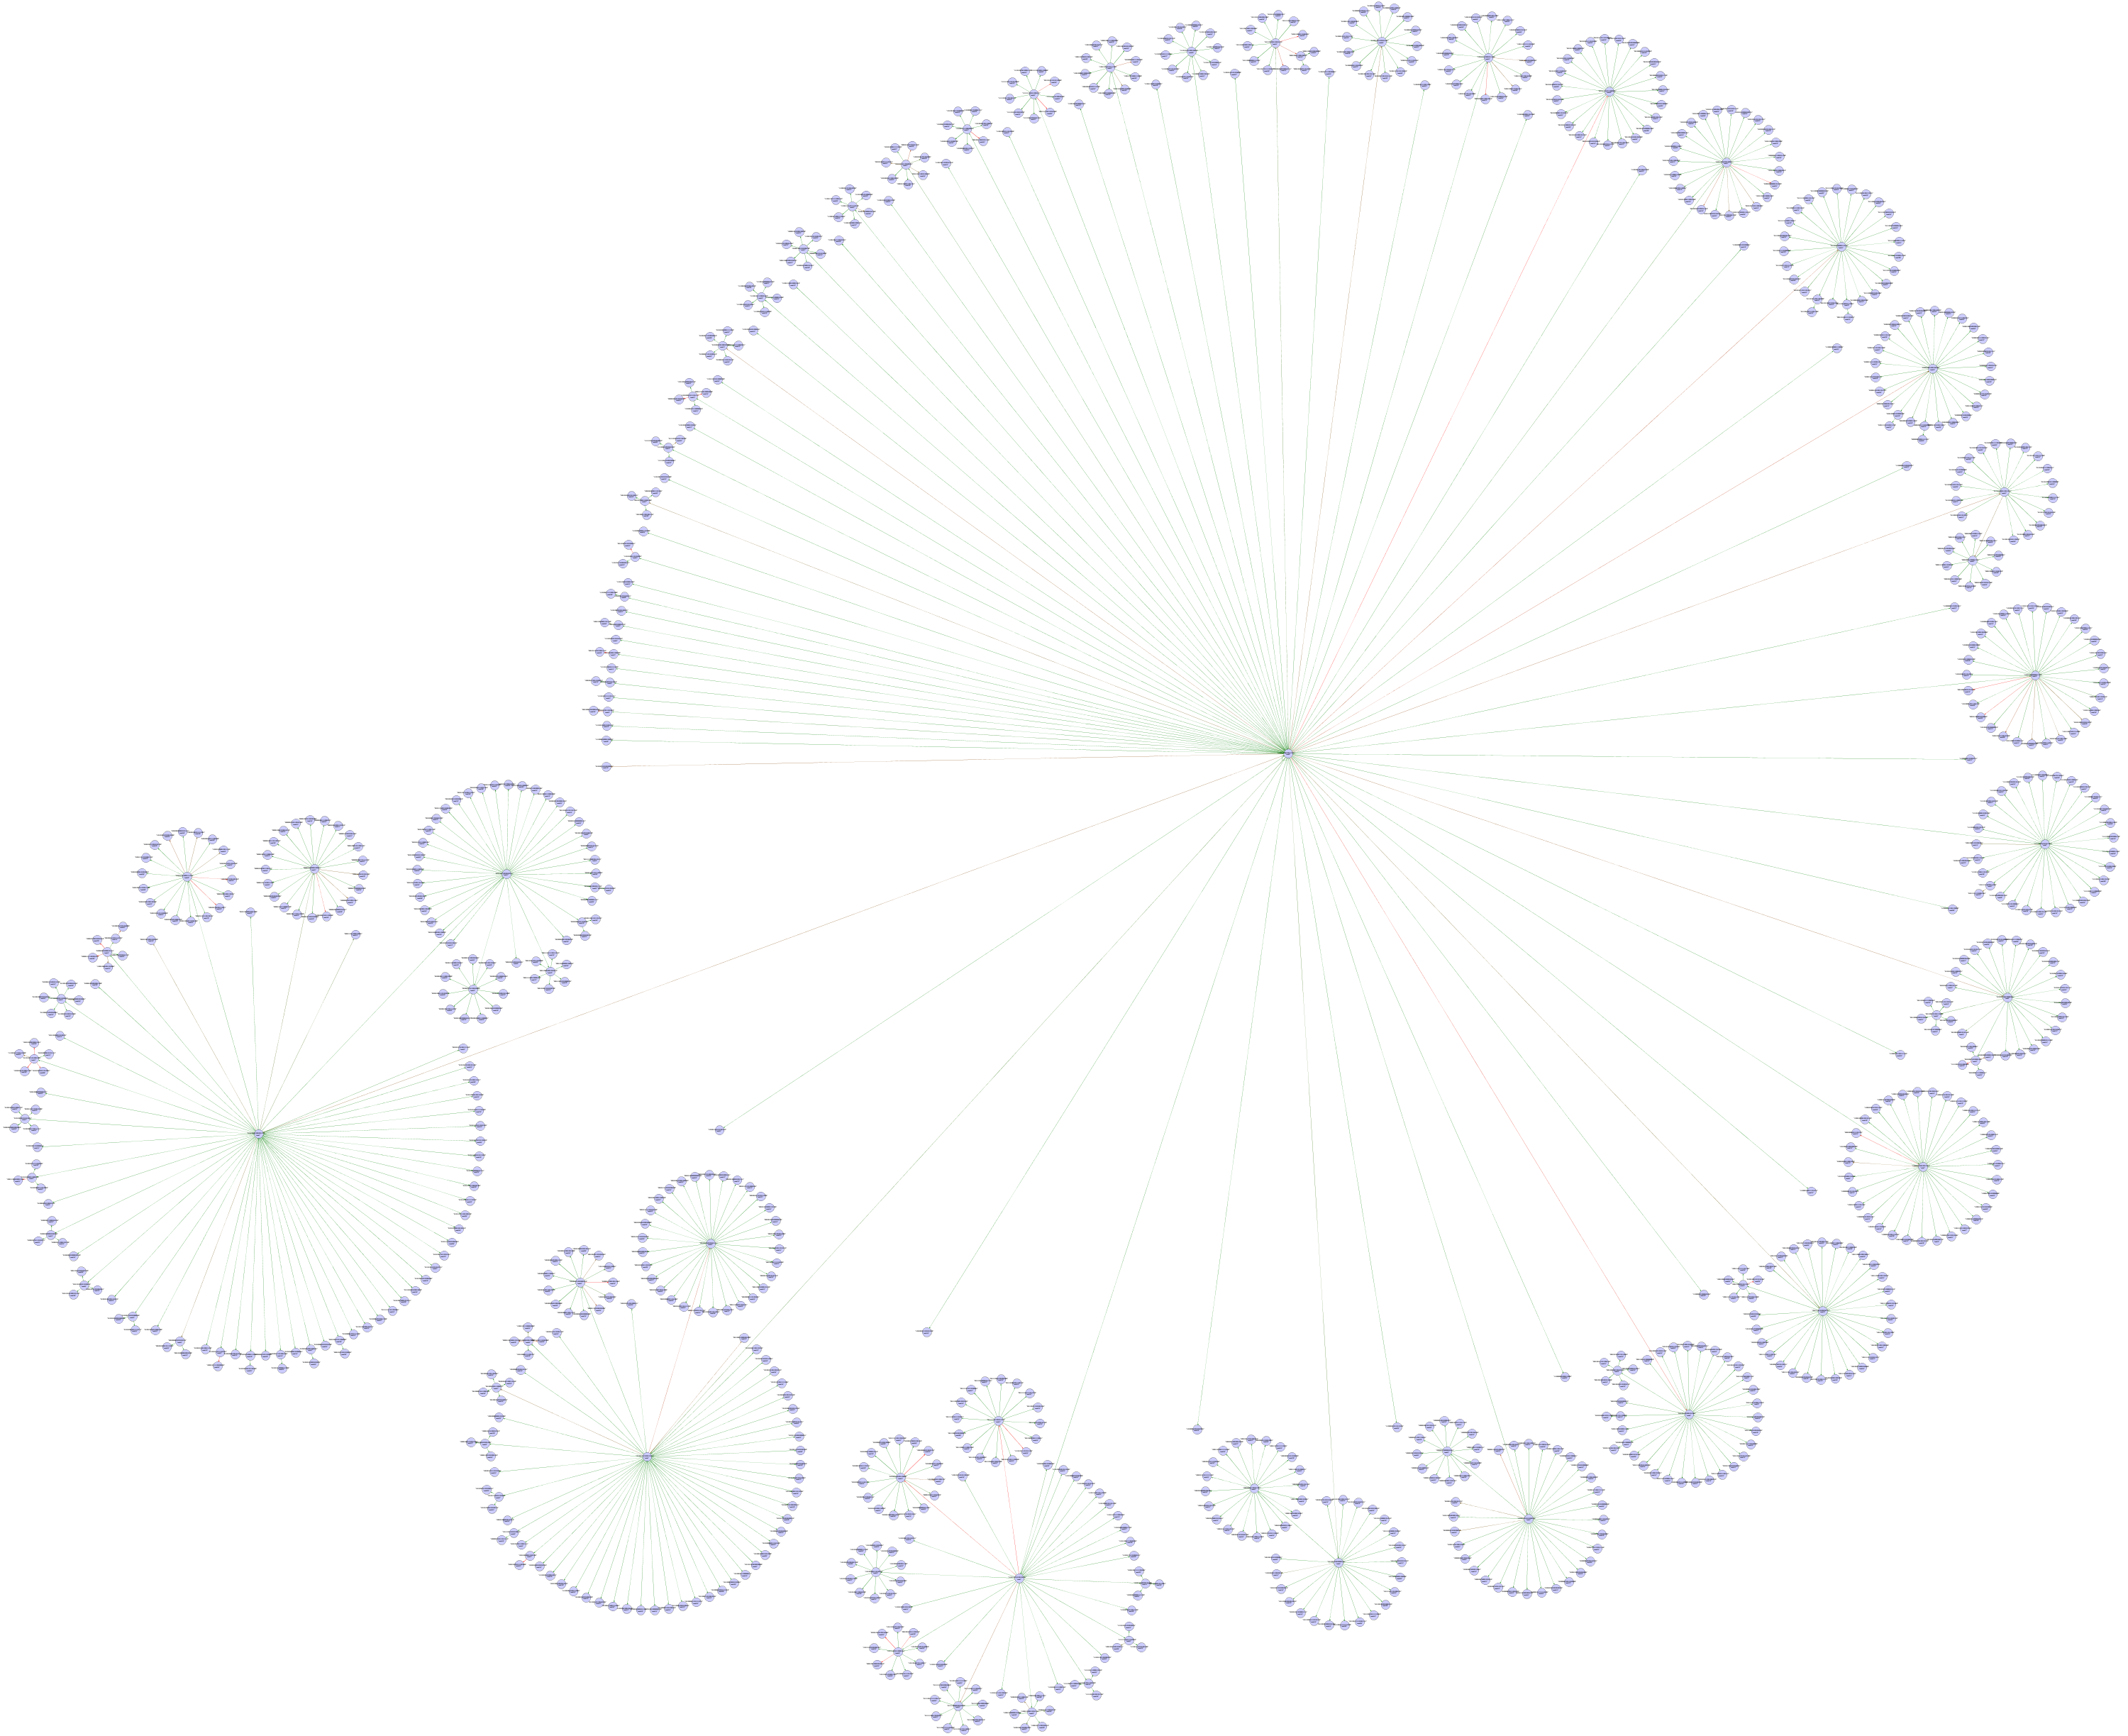
\includegraphics[width=15cm]{spanning.png}
   \caption{Spanning Tree}
\end{figure}

\pagebreak
\paragraph{The full topology} The most striking is the quasi division in the middle of the clew.
This is the ``first bit border'', the division between keys which start with a zero bit and those which start with a one bit.
The first is the most important bit as it influences the xor distance the most.

Darker/smaller nodes have joined the network later, brighter/bigger nodes are relatively old.
Note that in the two partitions of the network, the nodes are nicely mixed and distributed.
The graph comprises 500 nodes and 11,000 edges which gives a decent per node routing table of 22 entries.
This shows that the self-organizing network topology is very efficient as the routing tables are relatively small and the number of hops is logarithmical.
For 1000 nodes, the number of edges is ca. 30,000 which makes full topology plots usually to cluttered to really see anything.
\begin{figure}[htbp]
   \includegraphics[width=15cm]{topology.png}
   \caption{Full Topology}
\end{figure}

\begin{figure}[htbp]
   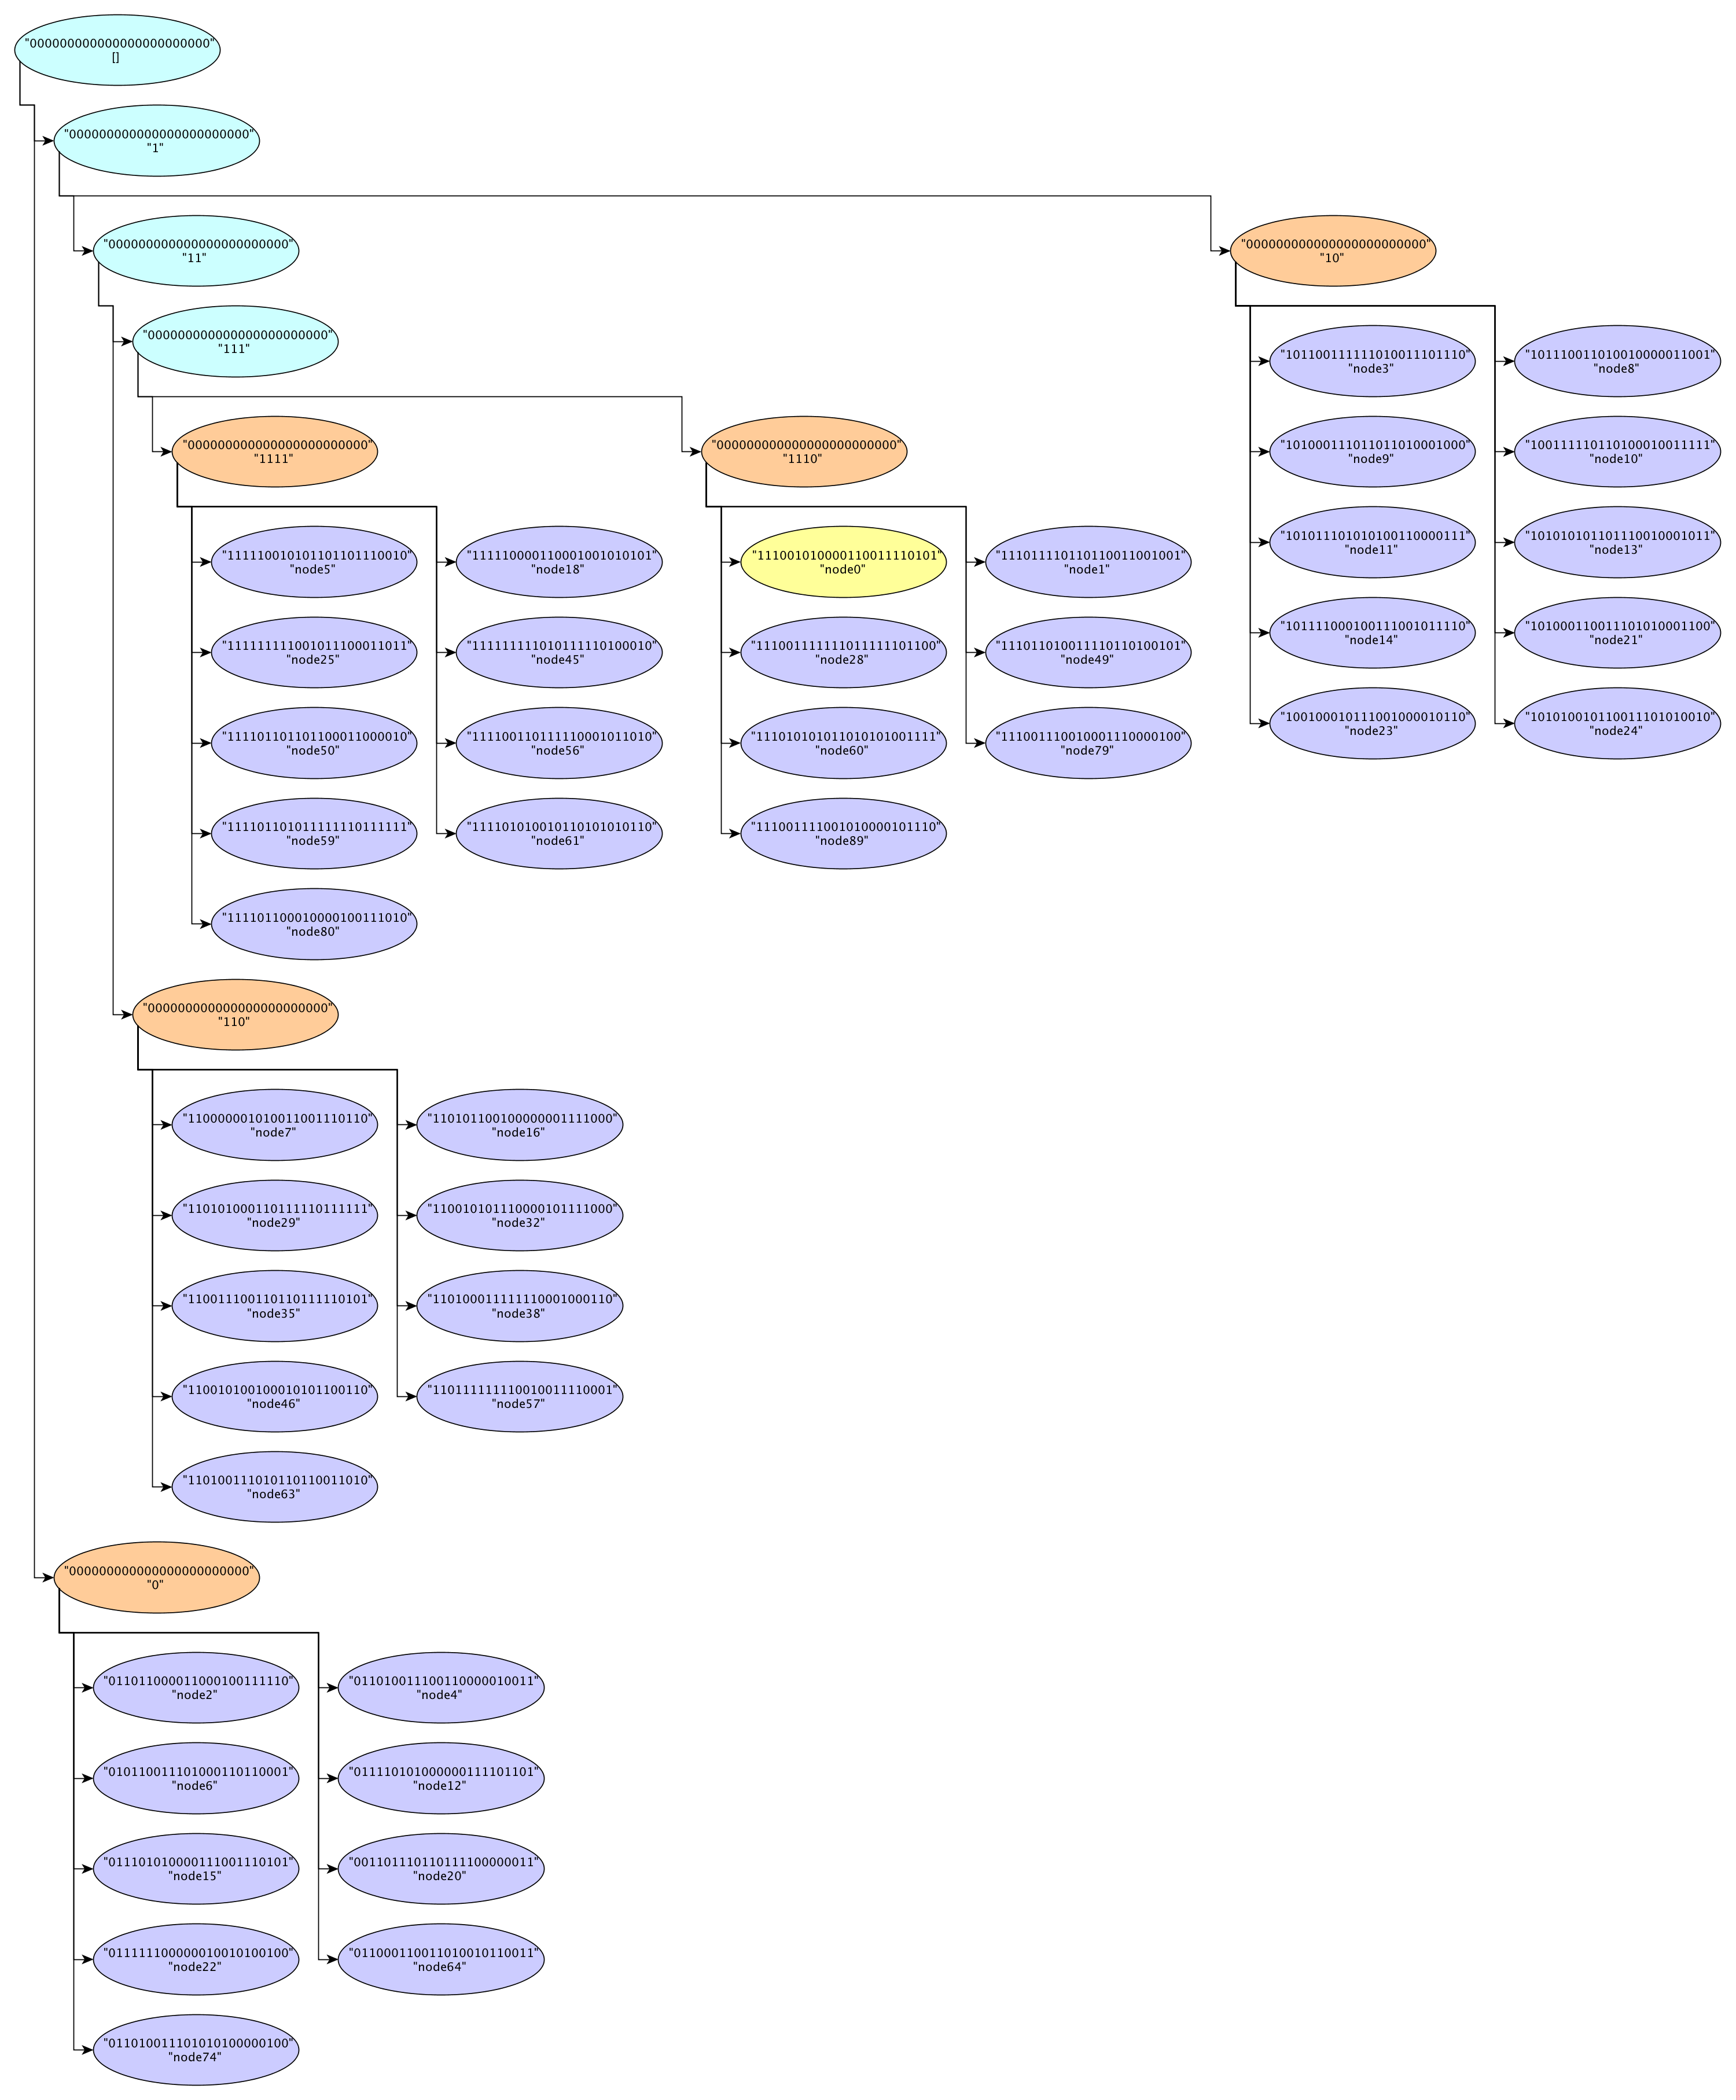
\includegraphics[width=15cm]{routingtable.png}
   \caption{A Routing Table}
\end{figure}

\pagebreak

\paragraph{Plain routing} This image shows the influence of hierarchical routing tables, i.e. ``the neighborhood-orientation'' of nodes.
The plot results from the network topology of 500 nodes which use a single bucket for all incoming contacts.
The edges are colored to display xor metric distance, from blue for close to red for distant.
Node colors are proportional to their size and these result from the order of creation.
Big/bright nodes have been in the network for a long time, small/dark nodes have joined later.
The only structure I can see is the preference for older nodes as these dominate the routing tables -- the remaining topology appears rather random.
\begin{figure}[htbp]
   \includegraphics[width=15cm]{plainrouting.png}
   \caption{Plain routing}
\end{figure}

\end{document}
